\documentclass[12pt]{article}
\setlength{\oddsidemargin}{0in}
\setlength{\evensidemargin}{0in}
\setlength{\textwidth}{6.5in}
\setlength{\parindent}{0in}
\setlength{\parskip}{\baselineskip}
\usepackage{amsmath,amsfonts,amssymb}
\usepackage{graphicx}
\usepackage{fancyhdr}
\usepackage{listings}
\usepackage{flexisym}
\usepackage[table]{xcolor}
\usepackage[utf8]{inputenc}
\graphicspath{ {./images/} }
\pagestyle{fancy}
%Code listing style named "mystyle"
\lstdefinestyle{mystyle}{
  basicstyle=\footnotesize,
  breakatwhitespace=false,
  breaklines=false,
  captionpos=b,
  keepspaces=false,
  numbers=left,
  numbersep=5pt,
  showspaces=false,
  showstringspaces=false,
  showtabs=false,
  tabsize=2
}
%"mystyle" code listing set
\lstset{style=mystyle}
\begin{document}
\lhead{{\bf CSCI 3403 \\ Homework 3} }
\rhead{{\bf Brennon Lee  \\ Fall 2018, CU-Boulder}}
\renewcommand{\headrulewidth}{0.4pt}
\vspace{-3mm}
\begin{enumerate}
% QUESTION 1
\item {The following cipher text was produced by the Caeser cipher: \\ \textbf{qeb mxpptloa fp nnwwnnw}}
  \begin{enumerate}
  \item {Use the Caeser cipher cryptanalyis techinique from lecture (Lecture 4 slides 13-16) to find the three most likely keys.} \\
    \textbf{Frequency of each letter is as follows: } \\
    \textbf{Q(16):0.05 E(4):0.05 B(1):0.05 M(12):0.05 X(23):0.05 P(15):0.15 \\ T(19):0.05 O(14):0.05 A(0):0.05 F(5):0.05 N(13):0.2 W(22):0.15 } \\

    \textbf{By writting a quick script that computes the correlation equation on slide 15 lecture 4, we find the top 3 most likely keys are: } \\
    \textbf{23 or 'X' with correlation value 0.032. 12 or 'M' with value 0.02675. And 1 or 'B' with value 0.028.}
  \item {Decrypt the message. You may use online tools from the Reading Assignment in the Data Security module.} \\

  \textbf{The decrypted message is: "\textit{the password is qqzzqqz}"} \\

  \item {Is the decryption key one of the three most likely keys from part A?} \\

  \textbf{Yes, the decryption key was in fact 23 or the letter 'X' which was one of our top three keys.}
  \end{enumerate}
\vspace{10pt}
% QUESTION 2
\item {\textbf{Review 2.4} List three approaches to message authentication. } \\

\textbf{The three approaches to message authentication is Symmetric Encryption, Hash Functions, and Public-Key Encryption}

% QUESTION 3
\item {\textbf{Review 2.7} What properties must a hash function have to be useful for message authentication? } \\
\textbf{Hash must be able to be applied to a block of any size.}\\
\textbf{Produces a fixed-length output.}\\
\textbf{H(x) is relatively easy to compute for any given x.}\\
\textbf{One-way or pre-image resistant.}\\
\textbf{Computationally infeasible to find $y \neq x$ that $H(y) = H(x)$}\\
\textbf{Collision resistant or strong collision resistance.}\\
\vspace{10pt}
% QUESTION 4
\item {\textbf{Review 2.9} List and briefly define three uses of a public-key cryptosystem? } \\
\textbf{Encryption \& Decryption - The sender can encrypt a message with the recipient's public key.} \\
\textbf{Digital Signature - The sender signs a message with their own private key.} \\
\textbf{Key Exchange - Two parties cooperate to exchange a session key. Approaches to this inlcude involving the private keys of one or both parties.} \\
\vspace{10pt}
% QUESTION 5
\item {\textbf{Review 2.10} What is the difference between a private key and a secret key?} \\
\textbf{The secrety key is used in symmetric (or conventional) encryption where both parties share a secret key. A private key is used in public-key (asymmetric) encryption. Where the public key is made public and the private key is only known to the user decrypting the message.}
\vspace{10pt}
% QUESTION 6
\item {\textbf{Problem 2.4}. Perhaps the simplest "serious" symmetric block encryption algorithms is the Tiny Encryption Algorithms (TEA). TEA operates on 64-bit blocks of plaintext using a 128-bit key. The plaintext is divided into two 32-bit blocks ($L_0,R_0$), and the key is divided into four 32-bit blocks ($K_0, K_1, K_2, K_3$). Encryptions involves repeated application of a pair of rounds, defined as follows for rounds $i$ and $i+1$:
\begin{center}
$L_i = R_{i-1}$\\
$R_i = L_{i-1} \boxplus F(R_{i-1}, K_0, K_1, \delta_i)$\\
$L_{i-1} = R_i$\\
$R_{i-1} = L_i \boxplus F(R_i, K_2, K_3, \delta_{i+1})$
\end{center}
where F is defined as
\begin{center}
$F(M, K_j, K_k, \delta_i) = ((M\ll  4) \boxplus K_j) \oplus ((M \gg 5) \boxplus K_k) \oplus (M+\delta_i)$
\end{center} }
and where the logical shift of x by y bits is denoted by $x \ll y;$ the logical right shift x by y bits is denoted by $x \gg y;$ and $\delta_i$ is a sequence of predetermined constants.
\begin{enumerate}
  \item {Comment on the significance and benefit of using the sequence of predetermined constants.} \\

  \textbf{The benefit and significance of using a sequence of constants is that a different constant can be used for encryption and decryption per round.}

  \item {Illustrate the operation of TEA using a block diagram or flow chart type of depiction.} \\

  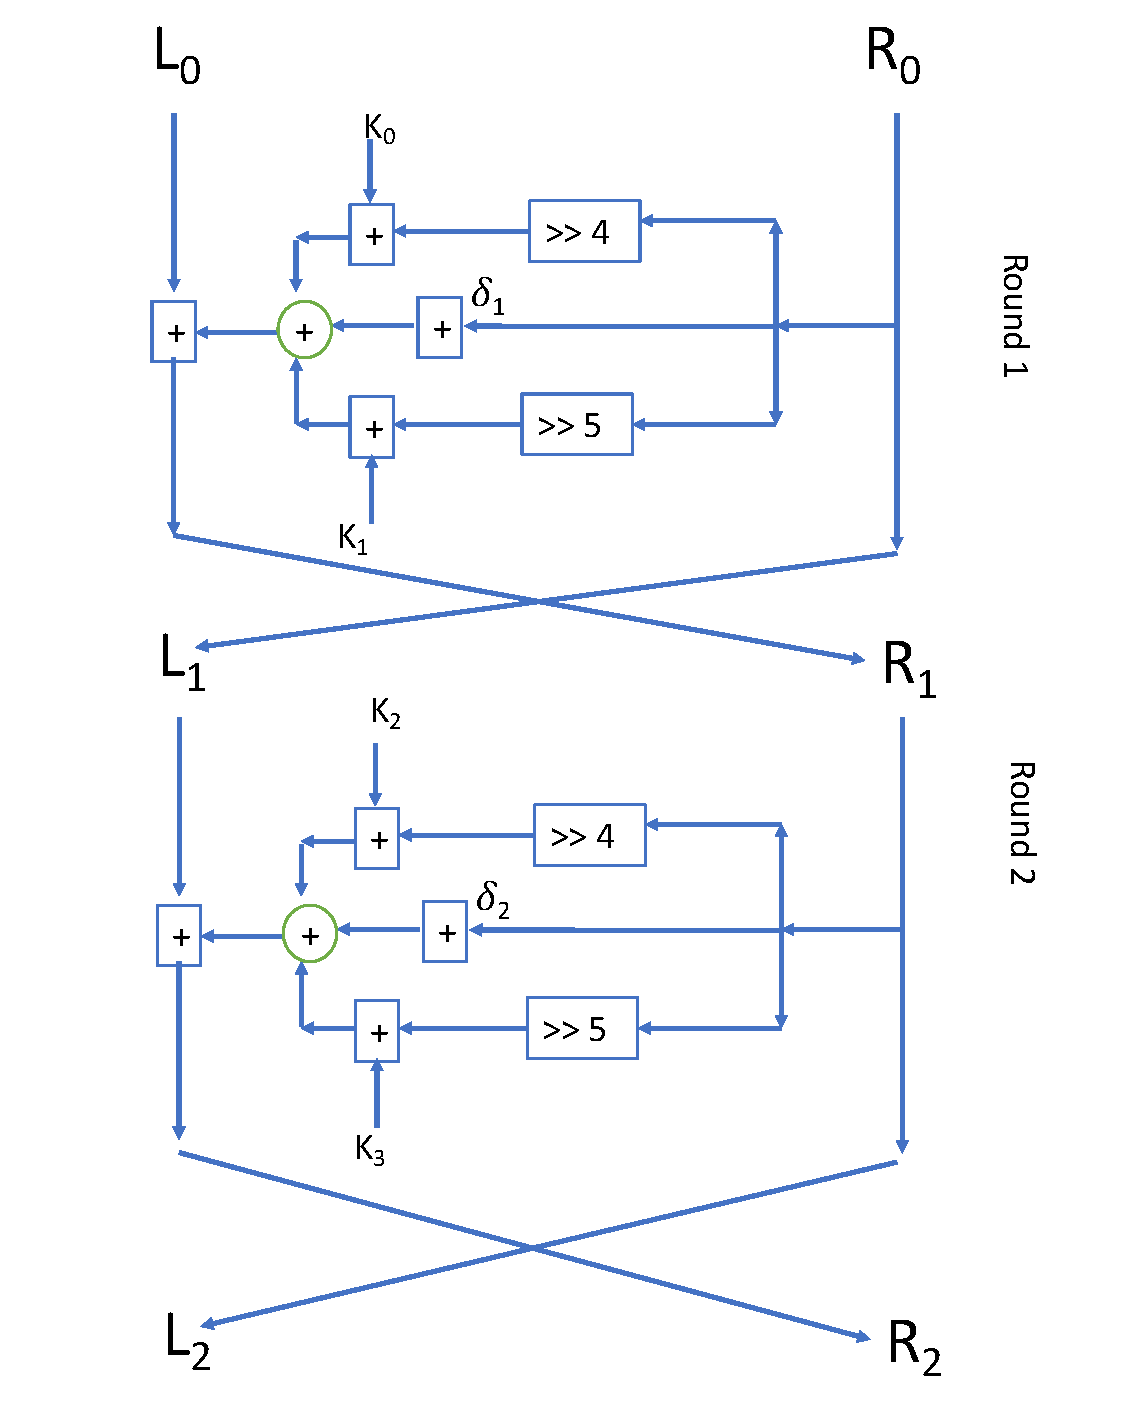
\includegraphics[scale=0.5]{encryption.pdf}

  \item {If only one pair of rounds is used, then the ciphertext consists of the 64 bit block $(L_2, R_2)$. For this case, express the decryption algorithm in terms of the equations.} \\

  \textbf{By solving the above equation in terms of the other variables, the decryption algorithm can be represented as:}
  \begin{center}
  $R_i = L_i + 1$\\
  $L_i = R_{i+1} \boxminus F(R_i, K_2, K_3, \delta_{i+1})$\\
  $R_{i-1} = L_i$\\
  $L_{i-1} = L_i \boxminus F(R_{i-1}, K_0, K_1, \delta_i)$
  \end{center}

  \item{Repeat part (c) using an illustration similar to that used for part (b).} \\

  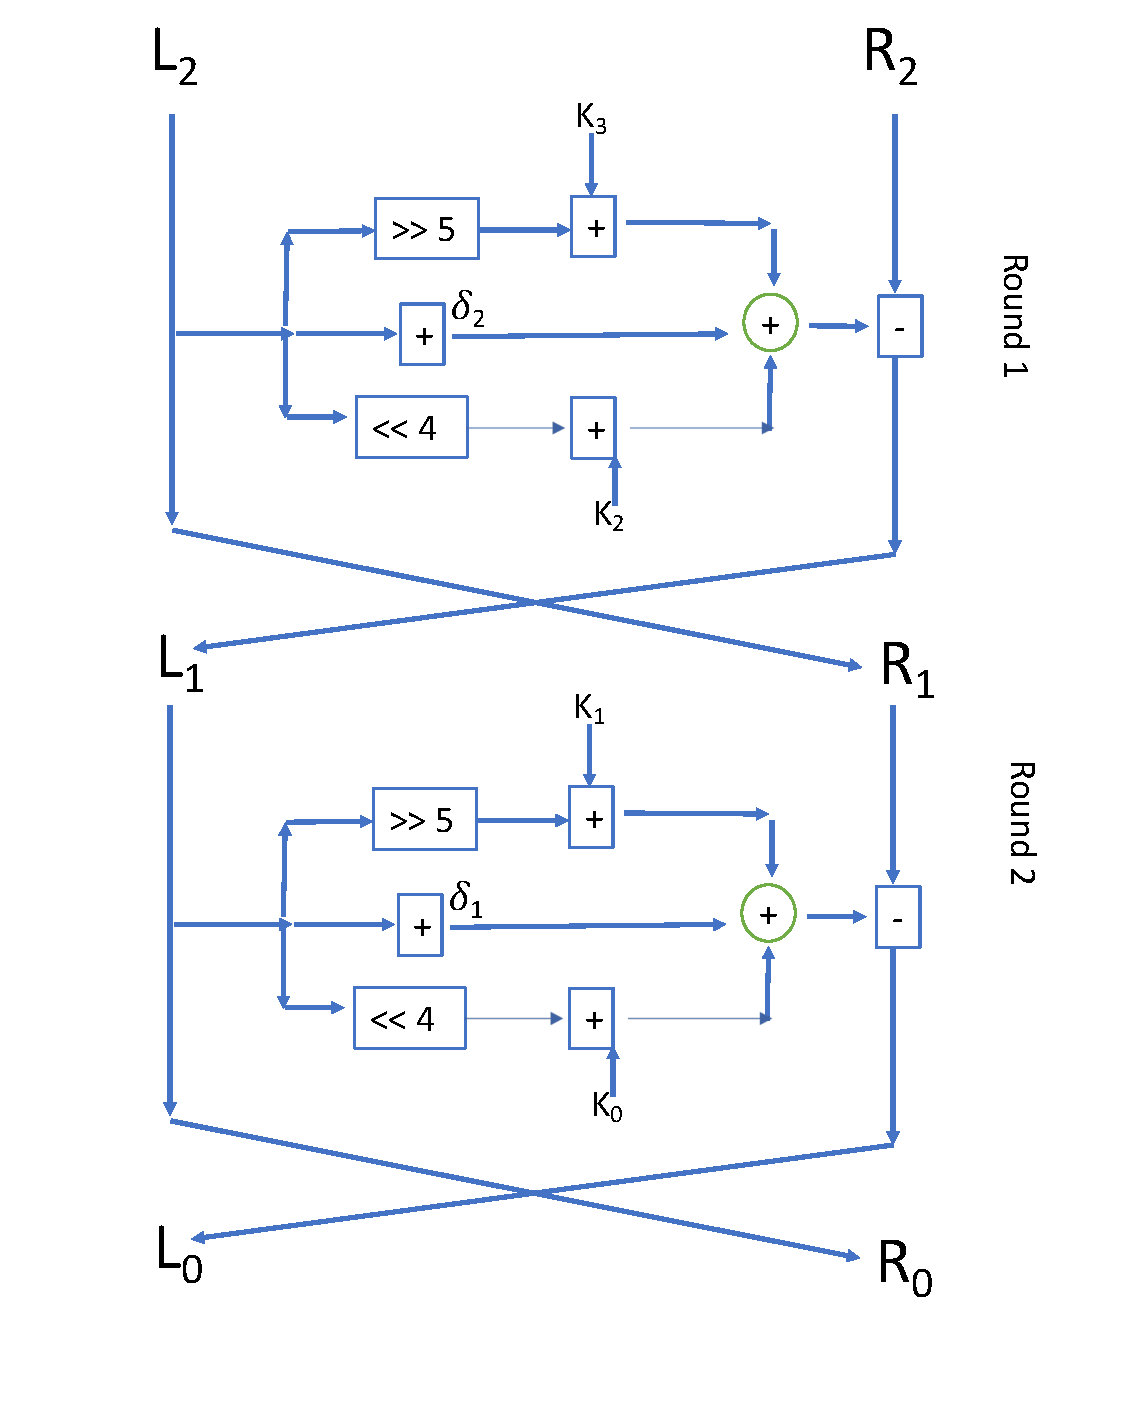
\includegraphics[scale=0.5]{decryption.pdf}

\end{enumerate}
\vspace{30pt}
% QUESTION 7
\item {\textbf{Problem 2.5}. In this problem, we will compare the security services that are provided by digital signatures (DS) and message authentication code (MAC). We assume Oscar is able to observe all messages sent from Alice to Bob and vice versa. Oscar has no knowledge of any keys but the public one in case of DS. State whether and how ($i$) DS and ($ii$) MAC protect against each attack. The value auth($x$) is computed with a DS or a MAC algorithm, respectively.}
\begin{enumerate}
\item (Message integrity) Alice sends a message x = "Transfer \$1000 to Mark" in the clear and also sends auth(x) to Bob. Oscar interscepts the message and replaces "Mark" with "Oscar". Will Bob detect this? \\

\textbf{In both cases, Bob can detect this change because the auth(x) wouldn't match x.}

\item (Replay)Alice sends a message x = "Transfer \$1000 to Oscar" in the clear and also sends auth(x) to Bob. Oscar obesres the message and signatiure and sends them 100 times to Bob. Will Bob detect this? \\

\textbf{No in both cases because the auth(x) will match x. The correct message just happens to be sent many times.}

\item (Sender Authentication with cheating third party) Oscar claims that he sent some message x with a valid auth(x) to Bob but Alice claims the same. Can Bob clear the question in either case? \\

\textbf{Case DS - Yes Bob can clear this because Alice's private key is only known to her and her public key will be authenitcated by Bob showing that the message could only have come from Alice with her private key.} \\
\textbf{Case MAC - Yes because Alice and Bob are sharing a secrete key that generates the auth(x). So Oscar's auth(x) will not match.}

\item (Authentication with Bob cheating) Bob claims that he received a message x with a valid signature auth(x) from Alice (e.g. "Transfer \$1000 from Alice to Bob") but Alice claims she has never sent it. Can Alice clear this question in either case?\\

\textbf{Case DS - Yes, Alice's private key is unique to only her to generate auth(x). And her public key will verify that the message came from her.} \\
\textbf{Case MAC -No, since both Alice and Bob both share the secret key, there is no way to dictate uniqueness between these two parties.}
\end{enumerate}
\vspace{40pt}
% QUESTION 8
\item {\textbf{Problem 2.6}. Suppose H($m$) is a collision-resistant hash function that maps a message of arbitrary bit length into an $n$-bit hash value. Is it true that, for all messages $x,x^'$ with $x\neq x^'$, we have $H(x)\neq H(x^')$? Explain your answer.} \\

\textbf{False, we are told that H(m) is collision-resistant hash function. So we know that it will be hard for two messages to have the same hash value. But it is still possible. Furthermore, our hash function is a fixed length so for an infinite amount of different messages, there cannot possibly be different hash values for each input. Therefore, it cannot be true that for all messages $x, x^'$ with $x \neq x^'$, we have $H(x) \neq H(x^')$}

\end{enumerate}
\end{document}
Search entries
